%%%%%%%%%%%%%%%%%%%%%%%%%%%%%%%%%%%%%%%%%%%%%%%%%%%%%%%%%%%%%%%%%%%%%%%%%%%%%%%
%%%%%%%%%%%%%%%%%%%%%%%%%%%%%%%%%%%%%%%%%%%%%%%%%%%%%%%%%%%%%%%%%%%%%%%%%%%%%%%
%%%%%%%%%%%%%%%%%%%%%%%%%%%%%%%%%%%%%%%%%%%%%%%%%%%%%%%%%%%%%%%%%%%%%%%%%%%%%%%
%%%%%%%%%%%%%%%%%%%%%%%%%%%%%%%%%%%%%%%%%%%%%%%%%%%%%%%%%%%%%%%%%%%%%%%%%%%%%%%
\section{The Dataset}
\label{sec:dataset}
%%%%%%%%%%%%%%%%%%%%%%%%%%%%%%%%%%%%%%%%%%%%%%%%%%%%%%%%%%%%%%%%%%%%%%%%%%%%%%%
%%%%%%%%%%%%%%%%%%%%%%%%%%%%%%%%%%%%%%%%%%%%%%%%%%%%%%%%%%%%%%%%%%%%%%%%%%%%%%%
%%%%%%%%%%%%%%%%%%%%%%%%%%%%%%%%%%%%%%%%%%%%%%%%%%%%%%%%%%%%%%%%%%%%%%%%%%%%%%%
%%%%%%%%%%%%%%%%%%%%%%%%%%%%%%%%%%%%%%%%%%%%%%%%%%%%%%%%%%%%%%%%%%%%%%%%%%%%%%%

\begin{figure}
    \centering
    \begin{subfigure}[b]{\textwidth}
	\centering
	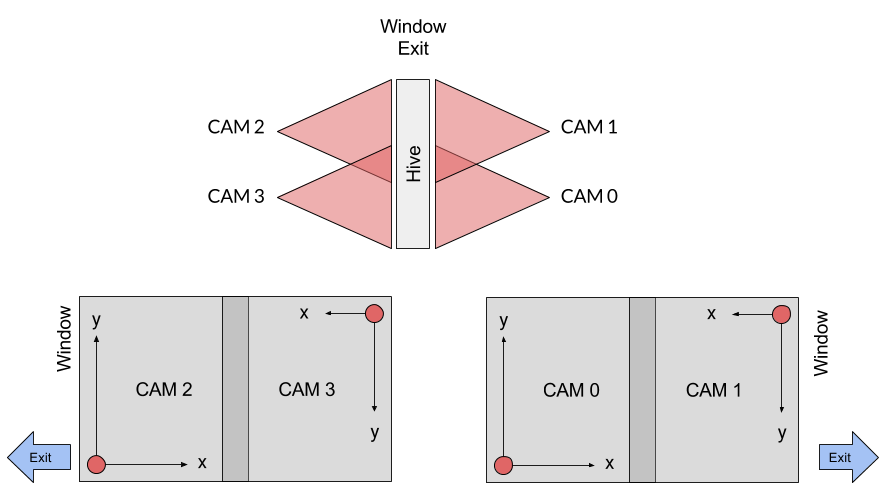
\includegraphics[width=0.8\textwidth]{Figures/setupCams}
	\caption[Camera setup]{\textbf{Camera setup} Each side of the honeycomb is filmed by two cameras. The two cameras per side do overlap, bees inside this are are detected from both cameras.}
	\label{fig:cams}
	\vspace{5mm}
    \end{subfigure}
    \begin{subfigure}[b]{\textwidth}
	\centering
	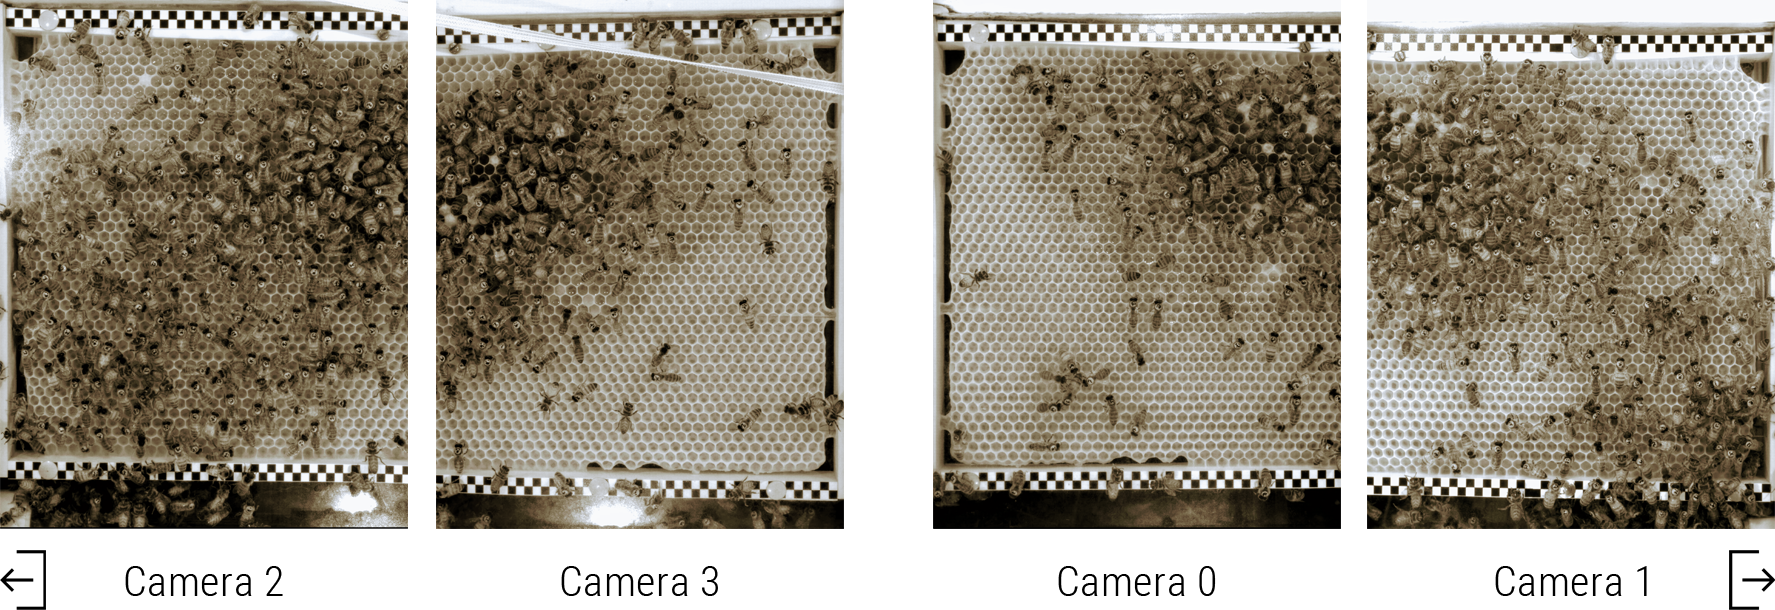
\includegraphics[width=0.65\textwidth]{Figures/beesClose}
	\vspace{5mm}
	\caption[Images for each camera]{\textbf{Images for each camera} Top: Side~A, bottom: side~B}
	\label{fig:veryclose}
    \end{subfigure}
 	\caption[Observation setup]{\textbf{Observation setup}}
 	\label{fig:obssetup}
\end{figure}

The dataset derives from high resoluted video files, that capture tagged honey bees of one colony in an one-frame observation hive.
The individuals of the colony, including about 3200 bees over a nine weeks period, were tagged with circular 12-bit markers (figure~\ref{fig:markers}, section~\ref{ch:intro}).
Two cameras per side filmed the complete honeycomb permanently.
Figure~\ref{fig:cams} illustrates the camera setup.
The \emph{recording period} lasted nine weeks (63 days), from 19.07.2016 until 19.09.2016, with some interruptions due to maintenance work and technical failures. [TODO: verlinken Appendix, uebersicht ueber gute und schlechte Zeiträume][TODO: Abbildung Aufnahmezeitraum]

All four cameras ($4000\times3000$ pixels) record $3.5$ frames per second. 
An image analysis pipeline~\cite{wario2015automatic} detects all bees in each frame.
The resulting detection data is stored in a binary file format.
An python library\footnote{The library is called \texttt{bb-binary} and is created by the Biorobotics Lab. It can be found on github: \url{https://github.com/BioroboticsLab/bb_binary}; Last accesed: 2106-02-16, 04:28PM} provides an frame-level access to those binary files.
The size of the dataset is $470$~GB, about $7.5$~GB of binary data per day.

The tagging period (67 days long) started on 28.06.2016 and lasted until 02.09.2016. Exactly $3.191$ bees were tagged. The young bees, which are raised in a separate hive, were tagged and then added to the observation hive, about noon each day. Figure~\ref{fig:tagging} shows the frequency of the tagging. The hatching day for each bee is documented; therefore the age of each bee at a particular point in time can be calculated.

[TODO: Begruendung des gewaehlten Zeitraumes: Funktionstüchtigkeit und Altersverteilung]
For further analysis, I chose three days (20.08., 22.08., and 24.08.) highlighted in figure~\ref{fig:period}.

\begin{figure}[htb]
	\centering
	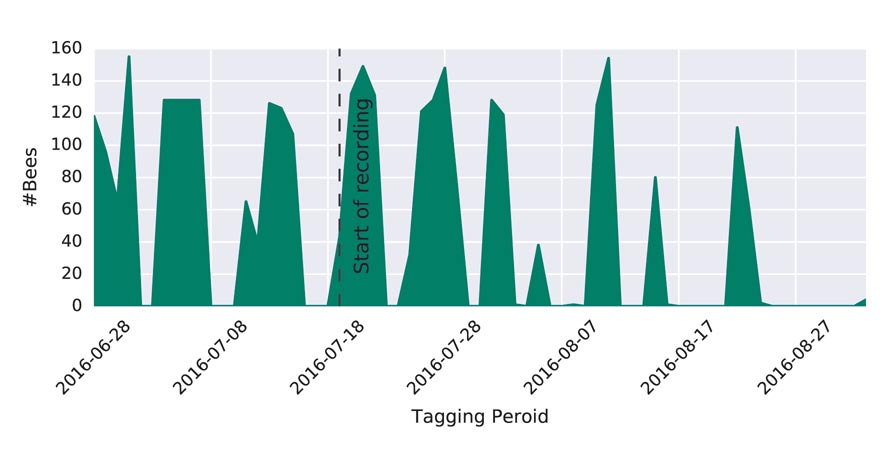
\includegraphics[width=1.0\textwidth]{Figures/tagging_period}
	\caption[Tagging frequency]{Tagging frequency: The bees were primarily tagged during the week. On average 48 bees were tagged each day, considering only tagging days, the average is about 91 ($\pm50$) bees (median 118). [TODO: combine with other image or make nicer!]}
	\label{fig:tagging}
\end{figure}

\begin{figure}[htb]
	\centering
	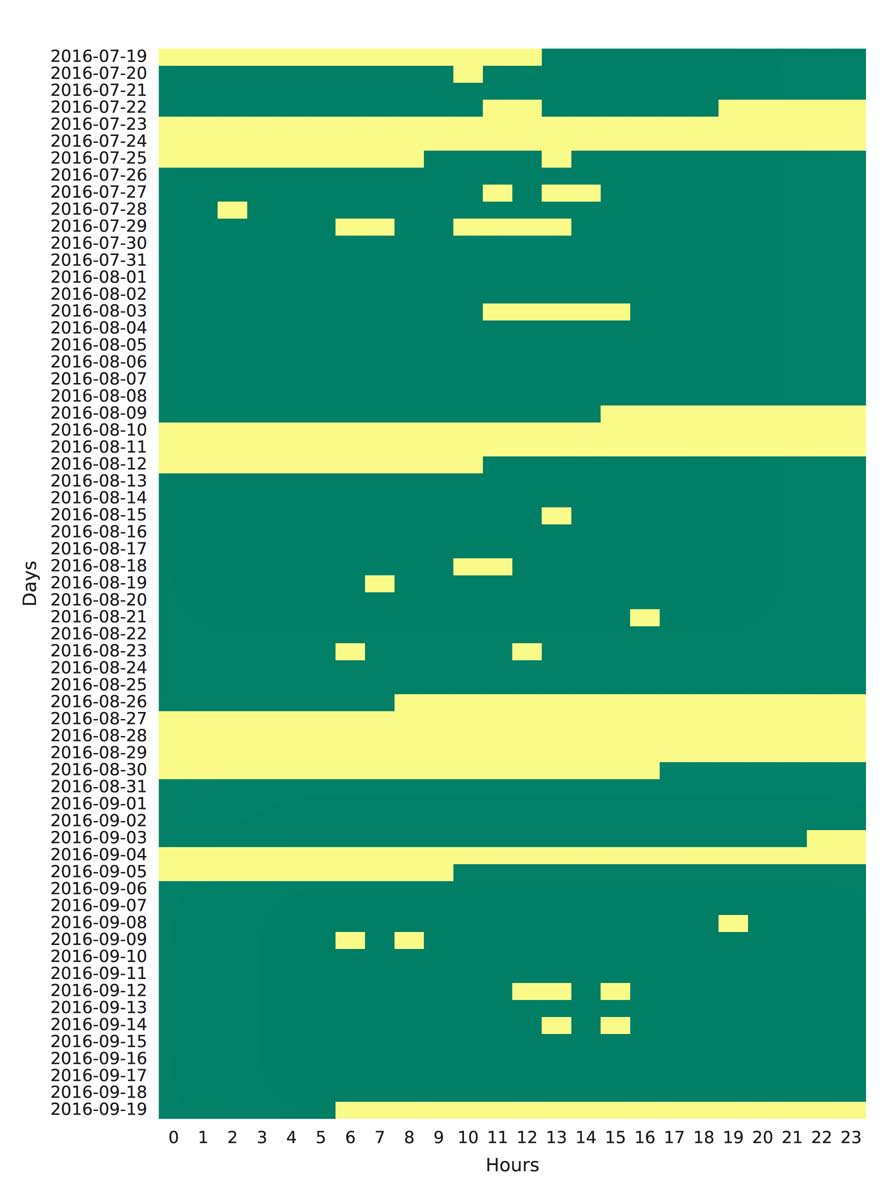
\includegraphics[width=0.4\textwidth]{Figures/recording}
	\caption[Recording season with maintainance and failures]{\textbf{Recording season with maintainance and failures} \emph{Green} indicates recording went without any big interruption; \emph{Yellow} indicates maintainance work or technical failures of one or all cameras. This is calculated using the expected number of files produced by each camera per hour. [TODO, reduzieren auf eine Info pro Tag (keine stuendliche aufloesung), kombinieren mit anzahl der getaggten bienen pro tag, und welchen Zeitraum hab ich nun verwendet], ausserdem Zeit von links nach rechts!, evtl. kein Datum, sonder Tage durchnummerieren}
	\label{fig:period}
\end{figure}

\clearpage
%%%%%%%%%%%%%%%%%%%%%%%%%%%%%%%%%%%%%%%%%%%%%%%%%%%%%%%%%%%%%%%%%%%%%%%%%%%%%%%
%%%%%%%%%%%%%%%%%%%%%%%%%%%%%%%%%%%%%%%%%%%%%%%%%%%%%%%%%%%%%%%%%%%%%%%%%%%%%%%
\subsection{Data Scheme}
\label{subsec:datascheme}
%%%%%%%%%%%%%%%%%%%%%%%%%%%%%%%%%%%%%%%%%%%%%%%%%%%%%%%%%%%%%%%%%%%%%%%%%%%%%%%
%%%%%%%%%%%%%%%%%%%%%%%%%%%%%%%%%%%%%%%%%%%%%%%%%%%%%%%%%%%%%%%%%%%%%%%%%%%%%%%
The data is organized in so-called \emph{frame containers}.
Each frame container corresponds to one video file of a single camera and consists of about $1024$ \emph{frames}. So the frame container specifies the camera (\emph{camId}), which took the video.
Each frame holds a list of bees, which were detected by the image analysis pipeline and is attributed with a \emph{timestamp}.

A bee \emph{detection} has, among others, the following attributes:

\begin{table}[!h]
\centering
\begin{tabular}{rl}
\textbf{xpos}: & $x$ coordinate of bee with respect to the image in pixel \\
\textbf{ypos}: & $y$ coordinate of bee with respect to the image in pixel \\
\textbf{decoded ID}: & decoded 12-bit ID \\
\\
\textbf{cam ID}: & ID of the camera ${0,1,2,3}$ \\
\textbf{timestamp}: & unix timestamp \\
\end{tabular}
\end{table}

The data can be accessed iterating on frame level, using a start and end time\-stamp, for specifying a time interval. The complete data scheme can be found on GitHub\footnote{\url{https://github.com/BioroboticsLab/bb_binary/blob/master/bb_binary/bb_binary_schema.capnp}; Last accessed: 2106-02-16, 04:46PM}. 

%%%%%%%%%%%%%%%%%%%%%%%%%%%%%%%%%%%%%%%%%%%%%%%%%%%%%%%%%%%%%%%%%%%%%%%%%%%%%%%
%%%%%%%%%%%%%%%%%%%%%%%%%%%%%%%%%%%%%%%%%%%%%%%%%%%%%%%%%%%%%%%%%%%%%%%%%%%%%%%
\subsection{ID Probabilities, Confidence Level, and Quality}
\label{subsec:confidence}
%%%%%%%%%%%%%%%%%%%%%%%%%%%%%%%%%%%%%%%%%%%%%%%%%%%%%%%%%%%%%%%%%%%%%%%%%%%%%%%
%%%%%%%%%%%%%%%%%%%%%%%%%%%%%%%%%%%%%%%%%%%%%%%%%%%%%%%%%%%%%%%%%%%%%%%%%%%%%%%

Twelve bits can encode the identity of 4096 bees.
Each bit of the decoded ID is not a one or zero, but represents a probability between $0$ and $255$, normalized to a value between $0$ and $1$. Therefore, a bit indicates the reliability of the image analysis pipeline.
I define the confidence $c$ for a bit $b$, analougus to Leon~\textcite[p.~14]{leon2016}, as $c(b)=2\cdot|b-0.5|$. The confidence of a decoded ID is, accordingly, the minimum of all twelve bit confidences.

The amount of data that remains for further processing and its correctness is highly dependent on the chosen level of confidence.

Additionally, I use the age information of the bees to check the quality of the remaining data. 
I examined (1) the number of detections and (2) the number of unique IDs, depending on the chosen confidence.
For each detection, the age was calculated. A detection with a negative age is counted as a wrong detection. I assumed that the number of wrong detections also occurred among detections with a positive age, but remained unseen; therefore I doubled the error, to be more accurate\footnote{On 26.07.2016, about half of the bee tags ($2014$ out of $4096$) were assigned. Because of this, that day was chosen to determine the effects of the level of confidence on data quality and the amount of remaining data.}. 

For (2), analogous a unique ID with a negative age is counted as a \emph{wrong} ID.

As expected, with an increasing confidence, the remaining data and unique IDs do decrease (figure~\ref{fig:remainingVSquality}). Also even though the number of wrong detections decreases steadily with an increasing confidence level, the number of wrong IDs only starts to decrease with a very high level of confidence.

With a confidence level of 100\%, 30.2\% of the remaining unique IDs are wrong (have a negative age), corresponding to only 2.5\% wrong detections of the remaining detections. Therefore, to obtain a more reliable dataset, wrong detections need to be filtered out, independently of the confidence value.

\begin{figure}
    \centering
    \begin{subfigure}[b]{0.45\textwidth}
        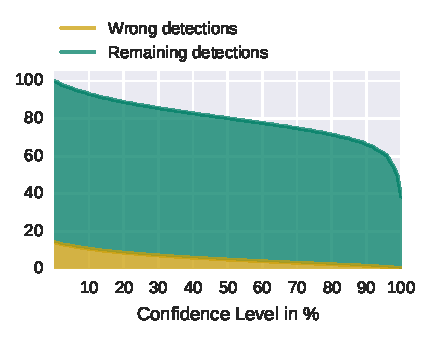
\includegraphics[width=\textwidth]{Figures/detectionsWrongConf}
        \caption[Detections]{ \textbf{Detections}}
        \label{fig:detections}
    \end{subfigure}
    \begin{subfigure}[b]{0.45\textwidth}
        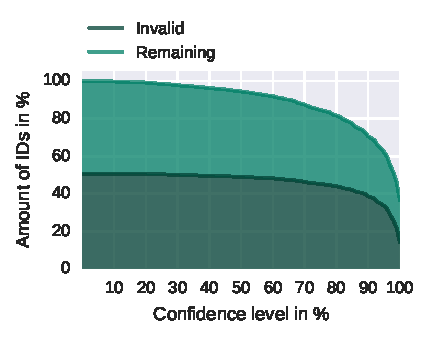
\includegraphics[width=\textwidth]{Figures/idsWrongConf}
        \caption[IDs]{\textbf{IDs}}
        \label{fig:ids}
    \end{subfigure}
 	\caption[Quality of detection and IDs]{\textbf{Quality of detection and IDs} \emph{Green} represents the number of remaining detections (from all, confidence 0\%) and remaining IDs (from 4096 possible IDs). \emph{Yellow} indicates the fraction of wrong IDs and detections in relation the remaining IDs and detections. (10~minute dataset, 26.07.2016, 4~p.~m., all cameras)}
 	\label{fig:remainingVSquality}
\end{figure}

 
\begin{table}[!b]
\colorbox{usethiscolorhere}{
\centering
\begin{tabularx}{\textwidth}{@{} r Y @{}}
	\textbf{Frame container} &
	A container for all frames, which belong to a specific video file of a certain camera.\\
	\textbf{Frame} &
	This includes all detections of one camera image, at a certain point in time.\\
	\textbf{Detection} &
	A detection of a bee at a certain point in time.\\
	\textbf{Decoded ID} &
	Identifyer of a bee consisting of 12 probability values, representing 12 bits.\\
	\textbf{Confidence} &
	Value between 0\% and 100\%).\\
	\textbf{ID} &
	The decimal representation of an decoded ID, after applying a certain confidence value.\\
	\textbf{Bee time series} & Binary sequence, indicating the absence and presence of a certain bee in a particular time interval.\\
	\textbf{Pair time series} & Binary sequence, indicating the absence and presence of two bees in a particular time interval.\\
\end{tabularx}
}
\end{table}

%%%%%%%%%%%%%%%%%%%%%%%%%%%%%%%%%%%%%%%%%%%%%%%%%%%%%%%%%%%%%%%%%%%%%%%%%%%%%%%
%%%%%%%%%%%%%%%%%%%%%%%%%%%%%%%%%%%%%%%%%%%%%%%%%%%%%%%%%%%%%%%%%%%%%%%%%%%%%%%
\subsection{Time Series of Bees and Bee Pairs}
\label{subsec:tracking}
%%%%%%%%%%%%%%%%%%%%%%%%%%%%%%%%%%%%%%%%%%%%%%%%%%%%%%%%%%%%%%%%%%%%%%%%%%%%%%%
%%%%%%%%%%%%%%%%%%%%%%%%%%%%%%%%%%%%%%%%%%%%%%%%%%%%%%%%%%%%%%%%%%%%%%%%%%%%%%%

The dataset, is transformed to binary \emph{bee time series}, depicted in figure~\ref{fig:structure} (left and middle). A time series of a bee is a sequence of zeros and ones indicating the absence and presence of a bee over a specified time interval. 
I examined the effect the level of confidence has on the bee time serie.
As expected, with an increasing confidence level the average gap length decreases and the overall number of gaps increases (~\ref{fig:gaps}).

The number of gaps those bee time series have, is important, because in a later step I want to extract pairs of close bees, who are present at the very same time. I call those \emph{pair time series}, as shown in figure~\ref{fig:structure} (right). So a lot of gaps in bee time series, could lead to a lot of gaps in the pair time series.

\begin{figure}[htb]
	\centering
	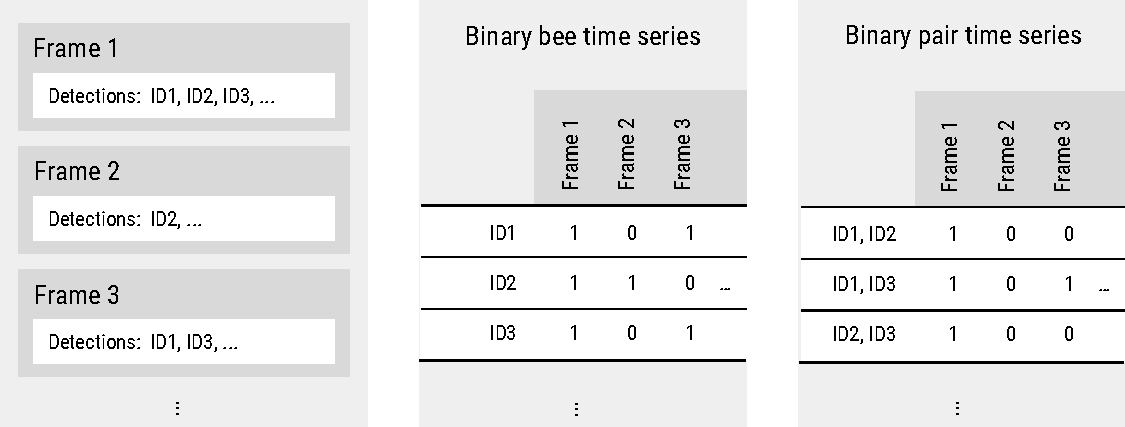
\includegraphics[width=1.0\textwidth]{Figures/structure}
	\caption[Structure of dataset]{\textbf{Structure of dataset} \emph{Left}: original dataset - containing a sequence of frames with bee detections; \emph{Middle:} binary bee time series - zero and one indicating absence and presence of the a bee; \emph{Right:} binary pairs time series - zero and one indicating the absence and presence of two bees in the same frame.}
	\label{fig:structure}
\end{figure}

\begin{figure}[htb]
	\centering
	\begin{subfigure}[b]{0.45\textwidth}
		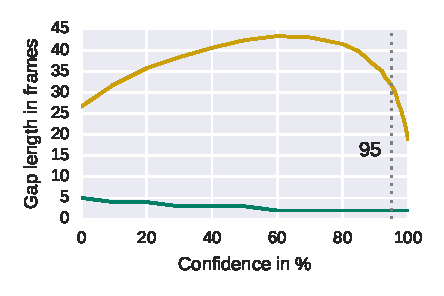
\includegraphics[width=\textwidth]{Figures/gaplen}
		\caption[Length of gaps]{\textbf{Length of gaps}}
		\label{fig:gaplen}
	\end{subfigure}
	\begin{subfigure}[b]{0.45\textwidth}
		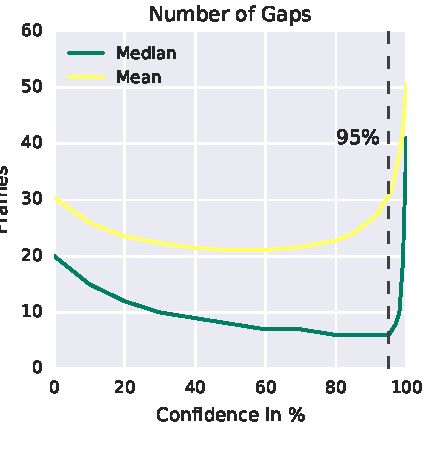
\includegraphics[width=\textwidth]{Figures/numgaps}
		\caption[Number of gaps]{\textbf{Number of gaps}}
		\label{fig:numgaps}
	\end{subfigure}
	\caption[Influence of Confidence Level on Gaps]{Influence of the confidence level of the length of gaps and number of gaps: With an increasing level of confidence the average gap length decreases and the number of gaps per bee series increases. (Dataset: 26.07.2016, 16:00-16:05)}
	\label{fig:gaps}
\end{figure}



%%%%%%%%%%%%%%%%%%%%%%%%%%%%%%%%%%%%%%%%%%%%%%%%%%%%%%%%%%%%%%%%%%%%%%%%%%%%%%%
%%%%%%%%%%%%%%%%%%%%%%%%%%%%%%%%%%%%%%%%%%%%%%%%%%%%%%%%%%%%%%%%%%%%%%%%%%%%%%%
\subsection{Detection Frequency Filter}
%%%%%%%%%%%%%%%%%%%%%%%%%%%%%%%%%%%%%%%%%%%%%%%%%%%%%%%%%%%%%%%%%%%%%%%%%%%%%%%
%%%%%%%%%%%%%%%%%%%%%%%%%%%%%%%%%%%%%%%%%%%%%%%%%%%%%%%%%%%%%%%%%%%%%%%%%%%%%%%
A good indicator, weather a bee is alive and present on a specific day, is the detection frequency of IDs. The hypothesis is: Bees with IDs who have a low detection rate are not physically present in the hive (do not exists at that day), due to detection errors of the image analysis pipeline.
To check this hypothesis, I investigate weather there is a correlation between age of the bee and detection frequency.

\begin{figure}[htb]
	\centering
	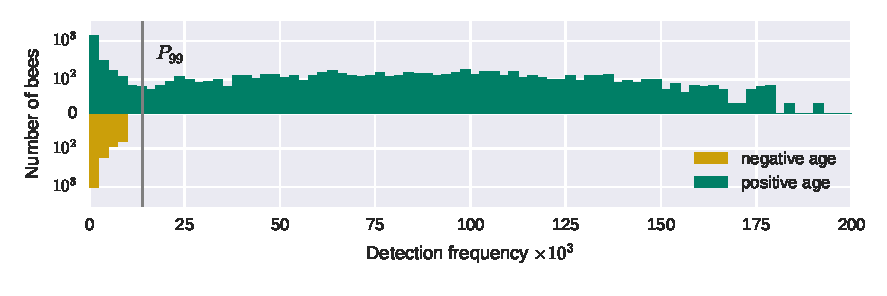
\includegraphics[width=1.0\textwidth]{Figures/filter}
	\caption[XXX]{\textbf{XXX} XXX}
	\label{fig:filter}
\end{figure}



IDs with a negative age are on average less detected than IDs with a positive age.

IDs who definately exists, but their age can to be determinded are excluded from the analysis completely. These are bees, who were tagged later~($n=10$)\footnote{id= [2,
	74,
	2045,
	3172,
	3764,
	3796,
	3827,
	3836,
	3844,
	3940]} and IDs whos detection frequency is absurd high but there age is unknown~($n=7$)\footnote{id=[has changed! 
	17,
	168,
	801,
	888,
	2045,
	2357,
	2607]}

For each analysis day the number of detections per ID is obtained, excluding the mentioned IDs above. The frequency distribution tells that, IDs with a negative age are detected less often ($704$ frames $\pm 65$)  than bees with a positive age ($36.603$ frames $\pm 2.345$). The cutoff is 99\% of the negative IDs distribution. All IDs with a detection frequency below $4737 \pm 644$ frames are discarded. A list with possible (valid) IDs is kept for each day. Using this list, faulty detections can be filtered out beforehand.

\clearpage
%%%%%%%%%%%%%%%%%%%%%%%%%%%%%%%%%%%%%%%%%%%%%%%%%%%%%%%%%%%%%%%%%%%%%%%%%%%%%%%
%%%%%%%%%%%%%%%%%%%%%%%%%%%%%%%%%%%%%%%%%%%%%%%%%%%%%%%%%%%%%%%%%%%%%%%%%%%%%%%
\subsection{Implications}
%%%%%%%%%%%%%%%%%%%%%%%%%%%%%%%%%%%%%%%%%%%%%%%%%%%%%%%%%%%%%%%%%%%%%%%%%%%%%%%
%%%%%%%%%%%%%%%%%%%%%%%%%%%%%%%%%%%%%%%%%%%%%%%%%%%%%%%%%%%%%%%%%%%%%%%%%%%%%%%
[TODO]
For further analysis I use the following days: 14.08.2016, 17.08.2016, 20.08.2016, 02.09.2016 with a confidence level of $95\%$. This period is chose because of XY.

Because bee time series contain a lot of short gaps (mean = 3, 95\% confidence), the inferring of edges (bees who are close to each other at the same time), should be not that strict, or at least variable. This has to be taken into acoount, when looking at spatialy close bees.